The RCT testbed has been designed and developed with the tools and libraries that are currently, as
the time of this writing, the state of the art. These tools are usually replaced by easier and more
powerful ones with time, and Higgs can benefit from these. When such a change is performed, normally
it will invalidate some of the documentation herein. Remember to write down the procedures and
descriptions to match the new devices and/or software.
When replacing a broken part, this chapter can be used as a guide for installing the new components.
The tools and libraries
in use are defined, as well as how they have been installed and configured, and a detailed description of the modules,
both hardware
and software.

%----------- 1 Mobile base ------------

\section{Mobile base}
\label{sec:devmanual_base}

\subsection{Disassembling the robot}
The main reason for disassembling the robot is to access the inside of the mobile base for repairs and updates. The remaining components can be accessed without major disassembling. The robot base has two black plates screwed to the red chassis with  a joint between them. This allows to access different parts of the robot without fully disassembling it. The front part of the robot is where the motors are placed and the inner on board computer can be fitted. No computer is currently installed inside so it will rarely need servicing. See section \ref{sec:disassembling_laser} to access it. The back part houses all power and control electronics and the batteries and can be reached disassembling the back methacrylate structure with the alluminium gantry. This is achieved by unscrewing all six bolts fixing it to the robot base. Be sure to unplug all necessary cords when taking it out. The robot base will power up but will not work correctly if the  multi-coloured ribbon cable is not properly connected to the black instrument panel of figure \ref{fig:photo_converter}.
\begin{figure}[ht]
\centering
 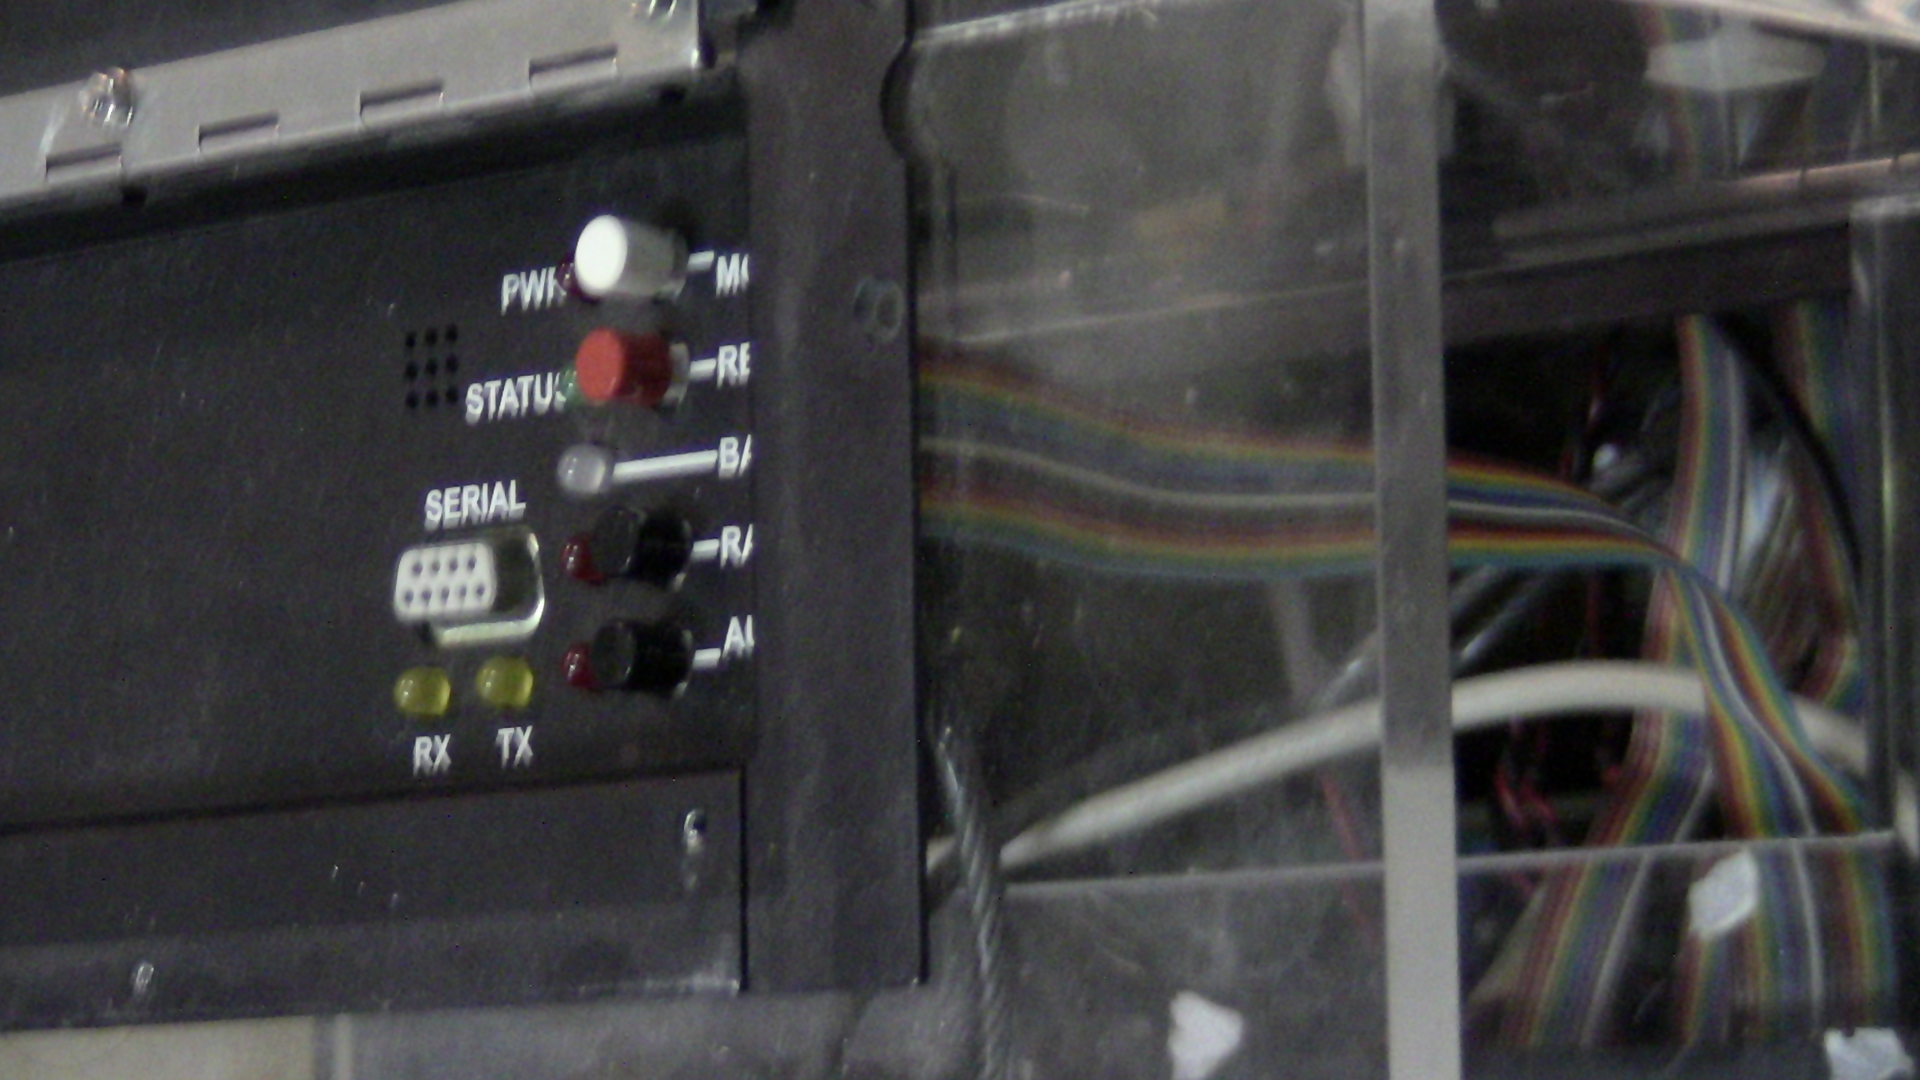
\includegraphics[width=0.8\textwidth]{figures/device_photos/multicolour_cable.jpg}
\caption{Robot base instrument panel.}
\label{fig:photo_converter}
\end{figure}


\subsubsection{Disassembling the laser}
\label{sec:disassembling_laser}
There are two ways to disassemble the laser. The first one removes the block composed of the laser sensor and the metacrylate structure that supports it. Get a number 5 allen wrench and unscrew the bolt placed under the laser, tiliting the latter upwards to reveal it. Then remove the two similar bolts on the other border of the alluminium plate that the first bolt was also holding. The methacrylate structure will be loose but do not take it off yet. Unplug the cords attached to the arduino board and the two data and power cords of the laser. Once all cables are released the structure can be lifted. Be careful not to damage the accelerometers when reassembling as its placement has been carefully crafted to fit between the laser structure and the arduino connection board. 

The second way allows for easier but more tedious disassembling. Remove the radio receiver of the GPS turning it as it was a huge bolt. Then unscrew the four bolts holding the upper methacrylate plate of the laser structure. Be careful with the weight of the devices fixed to this plate. This will leave the two walls standing to the sides of the laser. Looking from a robot point of view, the right wall can slide outwards releasing the laser from its side constraints. Take it out after unplugging the power and serial data cords. If further disassembling is required proceed as in the previous paragraph.

\subsubsection{Reaching the inside of the mobile robot.}
Once the top part of the mobile base is free from devices and structures both front and back inside parts of the robot can be reached unscrewing the littlest black bolts on the black plates. Additionally you can also remove the sonar sensors for reaching deeper inside the robot. There are four little vertical bolts inside the structure that holds each sonar array. Remove the ribbon cable prior to disassembling it.

In the back part of the robot reside the electronics in two layers. To access the bottom boards the top ones must be removed unscrewing the four small bolts situated behind the back wheels at the side of the robot and removing the sonar array so it can be slipped out.

\begin{figure}[htbp]
\begin{center}
 {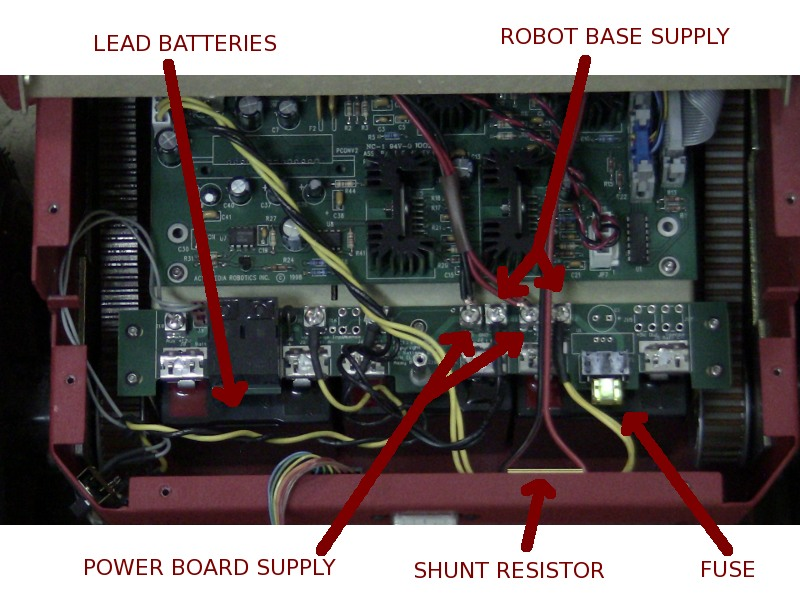
\includegraphics[width=\textwidth]{RCT_ModulesInsideRobotBase.jpg}}
\end{center}
\caption{Robot base front part disassembled.}
\label{fig:ModulesInsideRobotBase}
\end{figure}


\subsection{Firmware}
It is possible to update the firmware of the Mobile base, uploading it to the nonvolatile memory of the
Hitachi H8 microcontroller. Check the Pioneer 2 H8-Series Operations Manual. It is also possible to update
the tick count of the odometry.

%\subsection{CORBA servant}
%TODO


%----------- 2 Onboard computer ------------

\section{On-board computer}
\label{sec:devmanual_pc}

The onboard computer is the sony VAIO laptop running tUbuntu linux 10.04 with a RTAI kernel. The older onboard computer is a GENE board that was placed inside the mobile base with its own dc/dc regulator running WindRiver. See figure \ref{fig:RCT_old_gene}

\begin{figure}[htbp]
\begin{center}
 {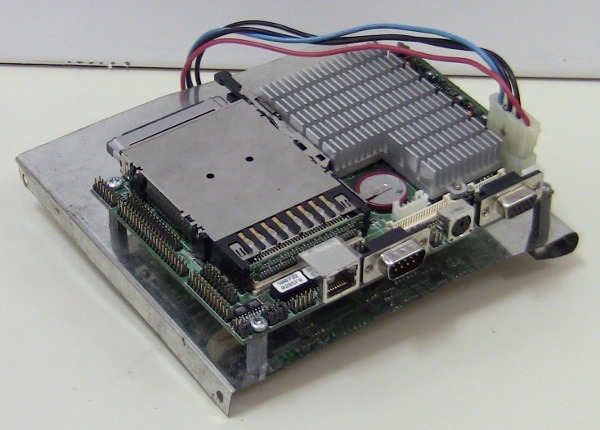
\includegraphics[width=0.7\textwidth]{RCT_ModulesVaioGene.jpg}}
\end{center}
\caption{The old onboard computer GENE}
\label{fig:RCT_old_gene}
\end{figure}

\subsection{Hubs and converters}
The onboard computer has two USB ports and one FireWire port among others. The FireWire port is used with the binocular camera. The arduino, GPS, laser, wrist and robot base all use serial RS-232 communication which is achieved using USB to RS-232 converters. There is a hub behind the power board with 4 USB ports to where the converters are plugged, either directly (two of them), with a short USB cable (i.e. the GPS) or has the converter chip embedded inside the device (i.e. the data acquisiton board). There is a lack of one serial converter for having all five devices working at the same time. Be sure to reconfigure the serial ports at \texttt{/etc/higgs/devices} when changing the connected devices, see \ref{sec:serial_links}.

\subsection{Real Time Operating System}
This section describes the steps that have been made for building and installing the Ubuntu RTAI operating system.
\begin{enumerate}
 \item Download and burn Ubuntu 10.04 LTS Desktop Edition, then install it like a standard Ubuntu installation.
The Long Term Support surname guarantees that this version will be supported for 3 years.
\item Install these packages: \texttt{libncurses-dev build-essential \\ kernel-package linux-source}
They are needed for building the kernel and generating a debian package.
\item Download and uncompress the vanilla linux kernel 2.6.32.11. The version must much exactly so the RTAI patch
can be applied smoothly. The linux kernel sources can be downloaded from \texttt{http://www.kernel.org/}.
\item Get the RTAI patch form \texttt{http://www.rtai.org/} As the time of this writing, the latest version was 3.8.1.
\item Apply the patch.
\begin{verbatim}
cd /pathtolinuxkernel2.6.32.11/
patch -p1 < /pathtortai/rtai-3.8.1/base/arch/x86/\
    patches/hal-linux-2.6.32.11-x86-2.6-0.3.patch
\end{verbatim} 
Be sure to use the patch for the exact kernel vanilla version, in this case 2.6.32.11, or errors and warnings
will arise. The \texttt{-p1} option removes the base directory form the path of the files inside the patch.
\item Configure the kernel. First, copy the ubuntu kernel config
\begin{verbatim}
 cp /lib/modules/`uname -r`/build/.config \
     /path_to_kernel-2.6.32.11
\end{verbatim} 
and run \texttt{make menuconfig} inside the root directory of the downloaded kernel sources. Look for the following options
and change them to the appropriate values: local version-append to -rtai.3.8.1-1; number of CPUs to 1; ACPI to no;
all power management features to no, module versioning support to yes, interrupt pipeline to yes.
The RTAI patch needs ACPI not to be supported by the kernel. As a consequence, no power management features will
work and the kernel will not be able to run the HALT instruction on shutdown.
\item Compile with \texttt{make}. This can last many hours.
\item Generate the debian package.
\begin{verbatim}
fakeroot
make-kpkg --initrd kernel_image kernel_headers
\end{verbatim} 
\item Go to the upper directory, where the packages are created, and install them with \texttt{dpkg -i *.dev}.
\end{enumerate}
Once the kernel is installed, reboot and start with the new kernel to check it con boot. Now it is time to
finish the installation compiling the realtime kernel modules and utilities.
\begin{enumerate}
 \item Go to the root directory of the RTAI source code and run \texttt{make menuconfig}. Select the number of
target cpu's with the same number as the kernel and write the path to the kernel sources.
\item \texttt{make} and as root \texttt{make install}.
\item Configure the libraries as root.
\begin{verbatim}
echo /usr/realtime/lib > /etc/ld.so.conf.d/rtai.conf
ldconfig
\end{verbatim} 
\item Add \texttt{/usr/realtime/bin} to the path of all users' .profile files.
\begin{verbatim}
 echo "PATH=$PATH:/usr/realtime/bin" > ~/.profile
\end{verbatim} 
\item Finally, check that the realtime extensions are working correctly. Go to \texttt{/usr/realtime/testsuite/kern/latency}
and run \texttt{./run}. If realtime is correctly installed, the last column should be all zeroes after 2-3 minutes.
\item Optionally, if space is low remove the packages and the source for the kernel and patch, or only the object files
with \texttt{make clean}.
\end{enumerate}


\subsection{OS Tweaks}
There are some modifications to be done to the Operating System to have Higgs' modules running flawlessly.

There must be a username called higgs and it must be a member of the dialout
group. Note also that by default the iptables firewall is enabled on many
distributions and it must be configured or disabled before CORBA clients can make calls to the
servants.

\subsubsection{Kernel modules}
\label{sssec:kernel_modules}
The linux kernel loads the serial modules for the converters at startup by default, but the order in which it does it is not the same on each bootup, so the serial device links must be checked on each bootup with this setup. The modules are the FTDI driver \texttt{ftdi\_sio.ko} and the pl2303 driver \texttt{pl2303.ko}. This inconvenience has been avoided by moving the kernel file objects from their standard placement at \texttt{/lib/modules/} to \texttt{/etc/higgs/modules}. The kernel tries to load the modules but fails because it can not find them where it expects them to be. The modules are loaded with the init scripts in a determined order. The following commands as root can be used to set up this behaviour on new installations:
\begin{verbatim}
cd /etc/init.d
echo "#!/bin/sh" > load_serial_modules
chmod a+x load_serial_modules
echo "insmod /etc/higgs/modules/pl2303.ko" \
 >> load_serial_modules
echo "insmod /etc/higgs/modules/ftdi_sio.ko" \
 >> load_serial_modules
ln -s /etc/init.d/load_serial_modules \
 /etc/rc3.d/S60load_serial_modules
\end{verbatim}
Replace \texttt{rc3.d} with the runlevel the OS starts with. You may instead prefer to modify the init script skeleton and give more functionality such as removal of the modules using the standard init V procedure such that loading and unloading the modules is done with \texttt{./load\_serial\_modules start/stop}.

\subsubsection{Daemon scripts}

The onboard portable computer is running many of the CORBA modules under
Linux. The base operating system has been modified slightly to run in an
unattended fashion.

Modifications made to the onboard computer:
\begin{itemize}
 % No more, as ACPI is disabled in linux RTAI.
  \item \texttt{/usr/bin/gnome\_power\_manager} has been renamed to \\
    \texttt{/usr/bin/gnome\_power\_manager.disabled}.
   This allows\footnote{This is not valid in Ubuntu RTAI as the ACPI subsystem is not functional. It is documented here in case other OS is used.} for the computer to run while it is on batteries and the screen is down.
   Otherwise the Vaio goes into suspend mode and no process can execute.
   To read the battery life do \\ \texttt{cat /proc/acpi/battery/BAT1/state} or
   \texttt{acpi -b}
 \item \texttt{/etc/init.d} The servants are configured to be managed by upstart. The config files determine which modules to load, when to restart and where to redirect the output (logs). See section \ref{ssec:module_config} for detailed description.
 \item \emph{restart\_servants} It is possible\footnote{This is not available when running the RTAI kernel.} to restart the servants by
   pressing the eject button on the Vaio, even with the lid down. This button
   will generate an ACPI event that will be processed by \texttt{acpid} using
   the configuration file \texttt{restart\_servants.conf} which in turn will
   call \\ \texttt{restart\_servants.sh} that will force the termination of the
   servants, which will be restarted by upstart. The
   configuration and script files go respectively under
   \texttt{/etc/acpi/events} and \texttt{/etc/acpi/actions}.
 \item The output of the commands are redirected to \\
   \texttt{/var/log/higgs/\$PROGRAM.log}
   Any problem associated to the execution of the modules may be diagnosed
   inspecting the logs in \texttt{/var/log/higgs/}, where all the output from the
   programs is registered. These files may grow big, so it has been created a
   logrotate config file for them (\texttt{higgslog}) placed in \texttt{/etc/logrotate.d/}.
\item MODULES: Removed pl2303 and ftdi\_sio kernel modules. They do not load with
   the same order on each bootup, so they are manually loaded by the inits scripts as described in \ref{sssec:kernel_modules}.
   The binaries have been moved from the original location to \texttt{/etc/higgs/modules}.
\end{itemize}


%----------- 3 Common libraries and module considerations ------------

\section{Common libraries and module considerations}
\label{sec:devmanual_common}
The RCT testbed may be controlled remotely by means of procedure calls to CORBA objects.
All of Higgs devices including the base platform have a CORBA interface definition that must be
used in order to remotely or automatically operate the robot. In this section these interfaces
are described in detail.

There are additional CORBA objects running in the on board computers that whilst not having direct control on Higgs'
physical devices, they do use the devices and provide useful, well-known and proved services.

\begin{figure}
\begin{center}
 {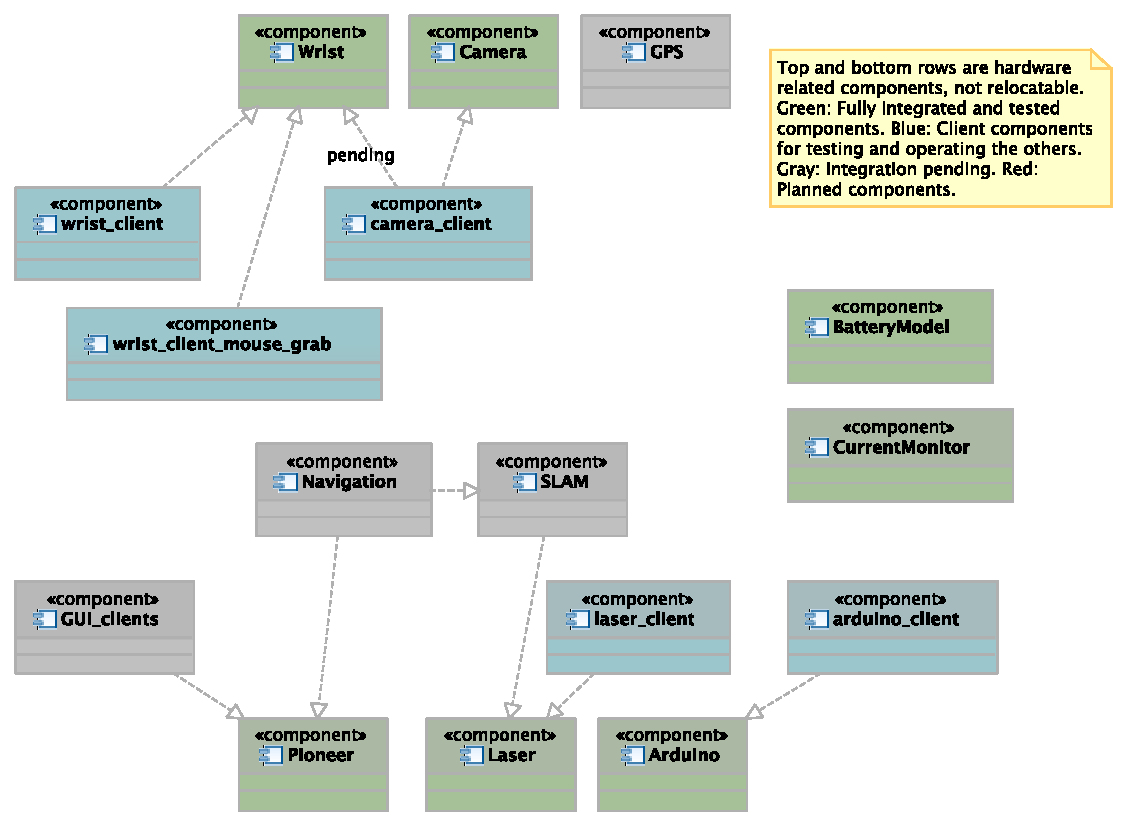
\includegraphics[width=1\textwidth]{RCT_ModulesCorbaComponents.pdf}}
\end{center}
\caption{General view of the CORBA modules in UML notation.}
\label{fig:ModulesCorbaComponents}
\end{figure}

The Java language requires that all CORBA interfaces are defined inside a module,
so all Higgs interfaces are defined inside the module \texttt{higgs}.


\subsection{ASLab servant utility functions for CORBA}
The same file \texttt{code/lib/CORBA\_utils.h} for easy creation of clients (see section \ref{sec:dev_client}) has also macros for servants.
A typical servant executable would be something like:

\begin{verbatim}
#include "implementation.h"
#include "CosNamingC.h"
#include "../../lib/CORBA_utils.h"

int main(int argc, char* argv[]) {
    CORBA_BEGIN_SERVER(argc, argv);

    implementation_t impl();
    higgs::implementation_t_var implvar = impl._this();

    CORBA_REGISTER_REFERENCE(implvar, "IMPL");
    CORBA_END_SERVER;
    return 0;
}
\end{verbatim} 
It is possible to use also \texttt{CORBA\_GET\_REFERENCE} in case other objects are needed.


\subsection{Module installation and configuration files}
\label{ssec:module_config}
The CORBA macros for the servants make use of the file
\begin{verbatim}
/etc/higgs/listen_endpoint.ip
\end{verbatim}
to configure the ip address where they should listen to, additionally to \\
the file \texttt{nameservice.ip} needed by clients.
Typically will contain the IPv4 address of the computer it is running in, in this case,
\begin{verbatim}
138.100.76.246
\end{verbatim}

Other config files are the device links at
\begin{verbatim}
/etc/higgs/devices
\end{verbatim}
Each module has this directory and the device file it uses hard coded in its source code.

Finally, they need an upstart config file. The upstart config file for the laser follows as example:
\begin{verbatim}
description "Upstart config file for the arduino servant"
author "Francisco J. Arjonilla Garcia"
start on started Naming_Service
respawn
script
	sleep 5
	date >> /var/log/higgs/laser.log
	su -l -c /usr/local/bin/laser_server higgs\
            >> /var/log/higgs/laser.log 2>&1
end script
\end{verbatim}
Other modules have different upstart config files. See each module source tree.
The Naming Service should start automatically. If not, an upstart config file must also be created for it. In either case, the endpoint must be specified in the parameters, i.e. manual execution:
\begin{verbatim}
./Naming_Service -ORBEndPoint\
    iiop://higgs2.disam.etsii.upm.es:9876
\end{verbatim}

The Java servant does not use the automatic NameService resolution mechanism provided by the C++ macros in \texttt{CORBA\_utils.h} and needs to have it specified as arguments when running it. Also, the next two lines must exist in the \texttt{.profile} file in the home directory of the user running the servant:
\begin{verbatim}
export PATH=/opt/jdk1.6.0_26/bin:${PATH}
export LD_LIBRARY_PATH=/usr/local/lib/
\end{verbatim}
Replace paths apropriately.

%----------- 4 I/O board ------------

\section{I/O board}
\label{sec:devmanual_io}

The I/O board manages the sensors and actuators that do not have a specific interface for connecting them to a computer. It has been implemented with an Arduino Mega board.
The devices controlled by the I/O board are:

\begin{itemize}
  \item Compass
  \item Accelerometers
  \item Battery sensors
  \item Laser pitch
  \item Power board
\end{itemize}

These devices are connected to the Arduino Mega commercial board through a
custom made extension board. The connector layout is shown in Figure
\ref{fig:ModulesArduinoExtensionPins}, and the connectors correspondence to
the devices in Table \ref{tab:ModulesArduinoExtensionPins}. The ribbon cable
connector  for controlling the powerboard is attached between the digital inputs 24 and 25.
Pin 0 (ground, red line on the ribbon cable) is closer to Pin22.

\begin{figure}[htbp]
\begin{center}
 {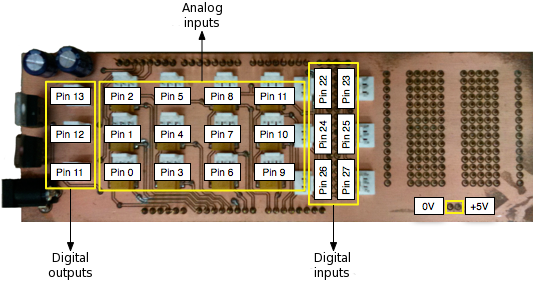
\includegraphics[width=1\textwidth]{RCT_ModulesArduinoExtensionPins.png}}
\end{center}
\caption{Connection diagram for compass board}
\label{fig:ModulesArduinoExtensionPins}
\end{figure}

\begin{table}
  \centering
  \begin{tabular}{|l|l|} \hline
    \textbf{Number} & \textbf{Device}\\ \hline \hline
    Pin0  & Not used \\ \hline
    Pin1  & Not used \\ \hline
    Pin2  & Not used \\ \hline
    Pin3  & Instrumentation current \\ \hline
    Pin4  & Instrumentation voltage \\ \hline
    Pin5  & Laser pitch potentiometer \\ \hline
    Pin6  & Motor current \\ \hline
    Pin7  & Motor voltage \\ \hline
    Pin8  & Accelerometer, X axis \\ \hline
    Pin9  & Not used \\ \hline
    Pin10 & Not used \\ \hline
    Pin11(Analog) & Accelerometer, Y axis \\ \hline
    Pin11(Digital) & Not used \\ \hline
    Pin12 & Not used \\ \hline
    Pin13 & Laser pitch servo \\ \hline
    Pin22 & Min pitch switch \\ \hline
    Pin23 & Max pitch switch \\ \hline
    Pin24 & Not used \\ \hline
    Pin25 & Compass \\ \hline
    Pin26 & Not used \\ \hline
    Pin27 & Not used \\ \hline
    Ribbon & Power board \\ \hline
  \end{tabular}
  \caption{Connector correspondence of the Arduino extension board with the
  devices.}
  \label{tab:ModulesArduinoExtensionPins}
\end{table}

\subsection{Tilt mechanism for the laser}
The laser sensor is housed inside a methacrylate structure with a joint that enables pitch movements on the laser. They are actuated by a servo placed just behind the laser, and by two end of stroke switches that limit the movements to safe values. To the left side of the laser, coaxial with the axis of rotation, there is a potentiometer that closes the loop for precise control of the rotation angle. The servo, switches and potentiometers are all controlled by the I/O board, which includes a PID control for the tilt programmed within its firmware. The details can be found in the PFC from Marcos Salom. % TODO: Falta cita bibliográfica.

Currently the PID feature has been disabled and the servo operates in an open loop fashion, using the end of stroke switches as a reference for rotation limits during initialization. The factors that motivated this decision are:
\begin{enumerate}
 \item The potentiometer is prone to errors due to mechanical hystheresis, worn out and temperature effects.
 \item There is a lot of functionlity that can be more useful than controlling the pitch of the laser. The effort has been so displaced elsewhere.
\item A better pitch angle sensor, such as an optic encoder, would justify buying a whole controlled actuator with integrated sensing and electronics.
\item The kinect sensor can partially substitute the laser.
\end{enumerate}


\subsection{Power board}
The I/O board and the power board have been connected with a ribbon cable that plugs to the doble row of pins of the extension board in the side of the I/O board. The ground connection has been stripped as the correspondent pin is not connected to ground in these pins. Common ground with the rest of the robot is achieved through the power connections that come from the batteries (Figure \ref{fig:ModulesInsideRobotBase}).


\subsection{Compass}
The compass is a solid state magnetism sensor placed next to the GPS antenna on
the aluminum bridge.
It was bought at www.superrobotica.com product reference CMPS03 S320160.
The connections are as follows, from bottom to top as shown
in figure \ref{fig:ModulesArduinoCompass}.
\begin{enumerate}
  \item VDD. To Arduino supply.
  \item SCL. To 5V with $47\Omega$ resistor.
  \item SDA. To 5V with $47\Omega$ resistor.
  \item PWM. To Arduino digital input.
  \item NC.
  \item Calibrate. To button in compass connector.
  \item 50Hz-60Hz. To GND.
  \item NC.
  \item GND. To Arduino supply.
\end{enumerate}

All connections including the calibration button are done inside the IDT
connector and protected by thermoadhesive. The button takes the calibration
input to ground when pressed.

\begin{figure}[htbp]
\begin{center}
 {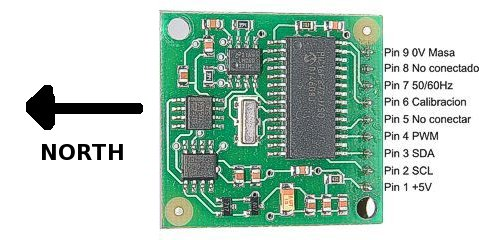
\includegraphics[width=.8\textwidth]{RCT_ModulesArduinoCompass.jpg}}
\end{center}
\caption{Connection diagram for compass board}
\label{fig:ModulesArduinoCompass}
\end{figure}

\subsubsection{Calibration instructions}
As noted in the manual of the compass, to calibrate it you have to press the
button  with the board heading perfectly well once in each direction:
North, West, South and East, no order required. It is already calibrated, so
there is no need to do it again.

The compass gives an output pulse of 1ms to 37 ms \@ VCC plus a fixed 65ms \@
GND. 1ms corresponds to $0^\circ$ and 37ms to $359^\circ$. 

The aluminum bridge does not interfere on the compass readings, but if the
robot is moving near steel structures they may be perturbed.


\subsection{Accelerometers}
There are two accelerometers encased on the same electronic board attached
horizontally with Velcro to the top cover of the robot base next to the I/O board.
They give a standard analog 0V to 5V signal and are connected directly to the
I/O board.

\subsection{Intensity/Voltage sensor}
There are two I/V sensors installed on board plus the battery status
indicator in Vaio accessible through the command line.
The two sensors can detect current and voltage of the Pioneer2AT batteries and
the instrumentation batteries. One operational amplifier per
battery has been used as a differential amplifier, as shown in Figure
\ref{fig:ModulesArduinoSensSch}. This design allows to detect small variations
in voltage of higher voltage than those of the working conditions of the
operational amplifier, specifically lower than $3.5V$, with the LM2904P
operational amplifier powered at $5V$. The voltage sensor is a scale down of the battery
voltage, which is then divided by the scale factor by software to recover the
true value. The gain is that of the differential amplifier. To read the
true current value, both the gain and the sensing resistor value must be
considered. See Table \ref{tab:ModulesArduinoDifferential} for the numerical values.
The printed circuit board is designed to fit into connectors 3,4,6 and 7 of the
Arduino extension board as an add-on module. The sensing resistors are placed
one inside the Pioneer2AT glued to the chassis under the back sonars
(figure \ref{fig:ModulesInsideRobotBase}) and the other one is in an aerial connection
on the battery cable immediately before the power board.


\begin{figure}[htbp]
\begin{center}
 {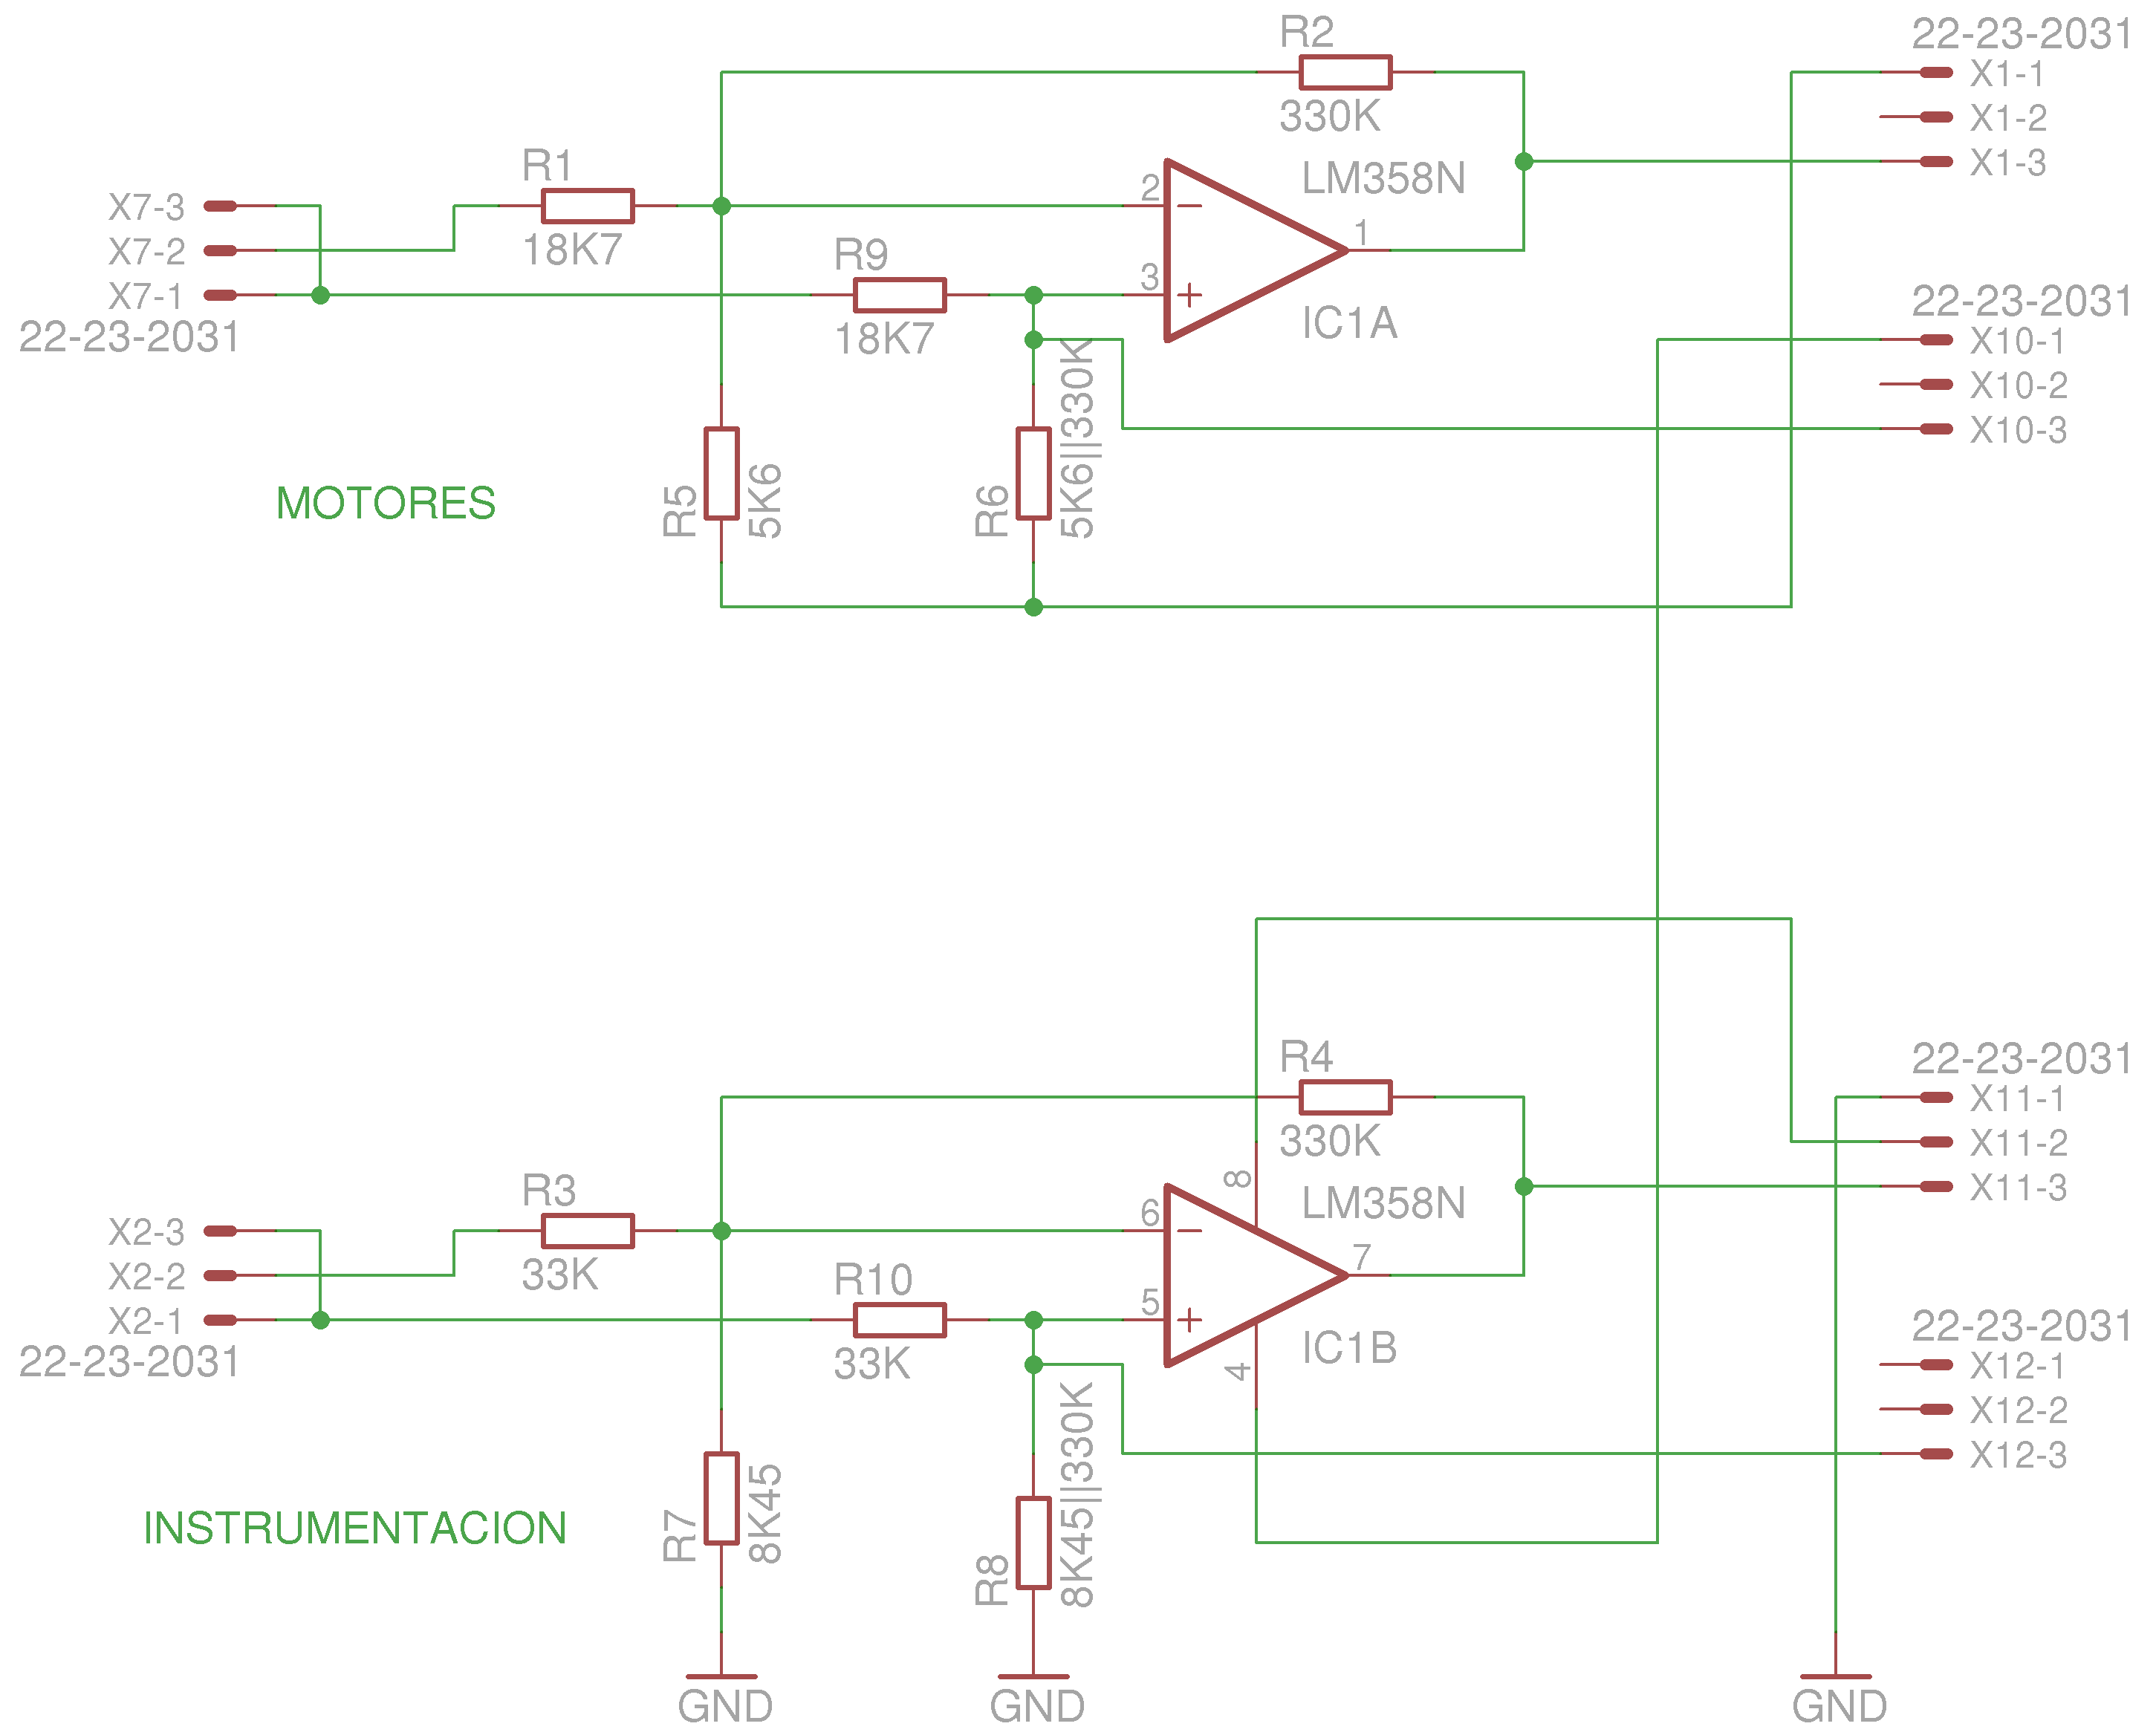
\includegraphics[width=.8\textwidth]{RCT_ModulesArduinoSensSch.png}}
\end{center}
\caption{Battery sensor schematic}
\label{fig:ModulesArduinoSensSch}
\end{figure}


\begin{figure}[htbp]
\begin{center}
 {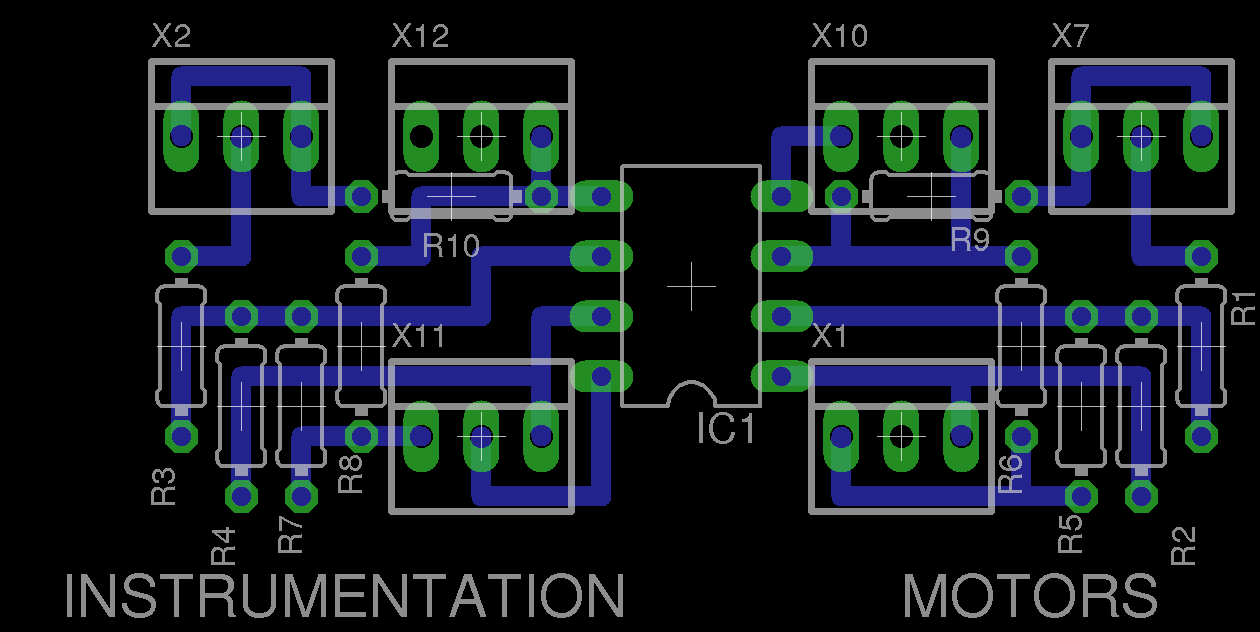
\includegraphics[width=.4\textwidth]{RCT_ModulesArduinoSensBrd.png}}
\end{center}
\caption{Battery sensor board layout}
\label{fig:ModulesArduinoSensBrd}
\end{figure}

Supposing ideal components, the output voltage given by the current sensor is
given by the formulae
\begin{equation}
U_0 = U^+\frac{R_{6}R_2}{R_9+R_6}(\frac{1}{R_1}+\frac{1}{R_2}+\frac{1}{R_5}) -
      U^-\frac{R_2}{R_1}
\end{equation} The condition that must be met for both references to be scaled down by the same
coefficient is that the relation of the resistor values
between the positive input and the negative input is
\begin{equation}
\frac{R_9}{R_6} = \frac{R_1}{R_2\parallel{}R_5}
\end{equation}
This way,
\[U_0 = \frac{R_2}{R_1}(U^+-U^-)\]
From this result we can observe that
there is great sensibility in the operation of the differential amplifiers. The
resistors from the negative input and the positive input must be of the same
value, of the same brand and of the same batch to give enough precision:
$R_9 = R1$ and $R_6$ physically being two
resistors in parallel: $ R_6 = R_2\parallel{}R_5 $.

\begin{table}
  \centering
  \begin{tabular}{|l||l|l|} \hline
    \textbf{Parameter} & \textbf{Instrumentation} & \textbf{Motors} \\ \hline \hline
	R1 & $33k\Omega$ & $18.7k\Omega$ \\ \hline
	R2 & $330k\Omega$ & $330k\Omega$ \\ \hline
	R5 & $8.45k\Omega$ & $5.6k\Omega$ \\ \hline
	R6 & $8.45k\Omega//330k\Omega$ & $5.6k\Omega//330k\Omega$ \\ \hline
	R9 & $33k\Omega$ & $18.7k\Omega$ \\ \hline
	Max sensing current & 6A & 17A \\ \hline
	Max differential input & 0.3V & 0.17V \\ \hline
	Gain & 10 & 17.647 \\ \hline
	Voltage scale factor & 0.1998 & 0.2275 \\ \hline
	Sensing resistor & $0.05\Omega$ & $0.01\Omega$ \\ \hline
  \end{tabular}
  \caption{Characteristics of the differential amplifiers for the battery
  sensors.}
  \label{tab:ModulesArduinoDifferential}
\end{table}

The current sensors will not work correctly while the batteries are charging.


\subsection{Servant and firmware}
The CORBA module for the I/O board has been written in the Java language whilst the test client in C++.
When the TurnOn and TurnOff methods are called, the appropriate device is turned
on/off and simultaneously, for the gps, laser, wrist and camera, the servant
that controls the device is killed from the arduino servant This only works if
the device servant is installed and running on the same machine as the arduino
servant, and will solve some issues on the protocol management that some of the
servants have with their device. The servant will then be restarted by the vaio
tools utility scripts.

Both the embedded program inside the I/O board and the Java servant communicate
through a USB data connection that gets converted to serial RS-232 by a FTDI chip in the Arduino board.
The I/O board starts the
communication protocol by sending all the parameters and sensor readings to the
servant, and then the servant optionally answers with the order.

The figures \ref{fig:ModulesArduinoClasses}, \ref{fig:ModulesArduinoInteraction},
\ref{fig:ModulesArduinoPC2A} and \ref{fig:ModulesArduinoA2PC} show the UML model
of the JAVA sources of the Arduino CORBA servant.

\begin{figure}[htbp]
\begin{center}
 {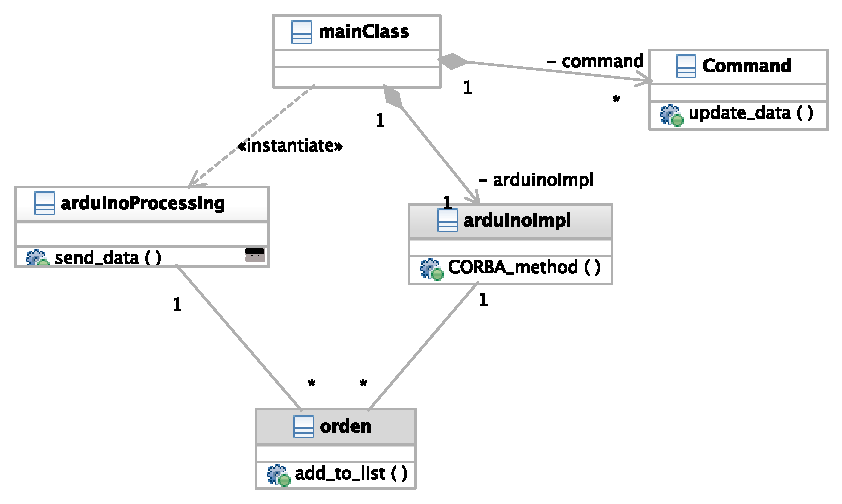
\includegraphics[width=1\textwidth]{RCT_ModulesArduinoClasses2.pdf}}
\end{center}
\caption{CORBA interface and classes used in the JAVA implementation.}
\label{fig:ModulesArduinoClasses}
\end{figure}

\begin{figure}[htbp]
\begin{center}
 {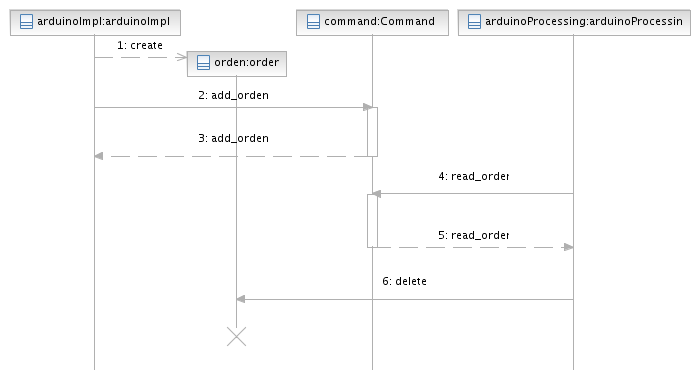
\includegraphics[width=1\textwidth]{RCT_ModulesArduinoInteraction.png}}
\end{center}
\caption{Interaction diagram for the Arduino CORBA module.}
\label{fig:ModulesArduinoInteraction}
\end{figure}

\begin{figure}[htbp]
\begin{center}
 {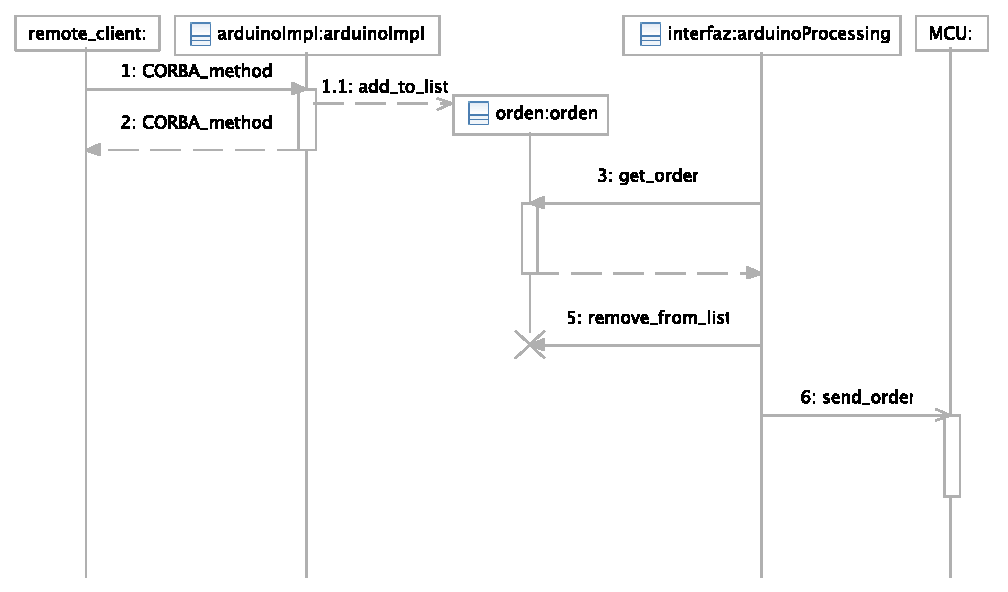
\includegraphics[width=1\textwidth]{RCT_ModulesArduinoPC2A.pdf}}
\end{center}
\caption{Sequence diagram for sending data to the i/o board.}
\label{fig:ModulesArduinoPC2A}
\end{figure}

\begin{figure}[htbp]
\begin{center}
 {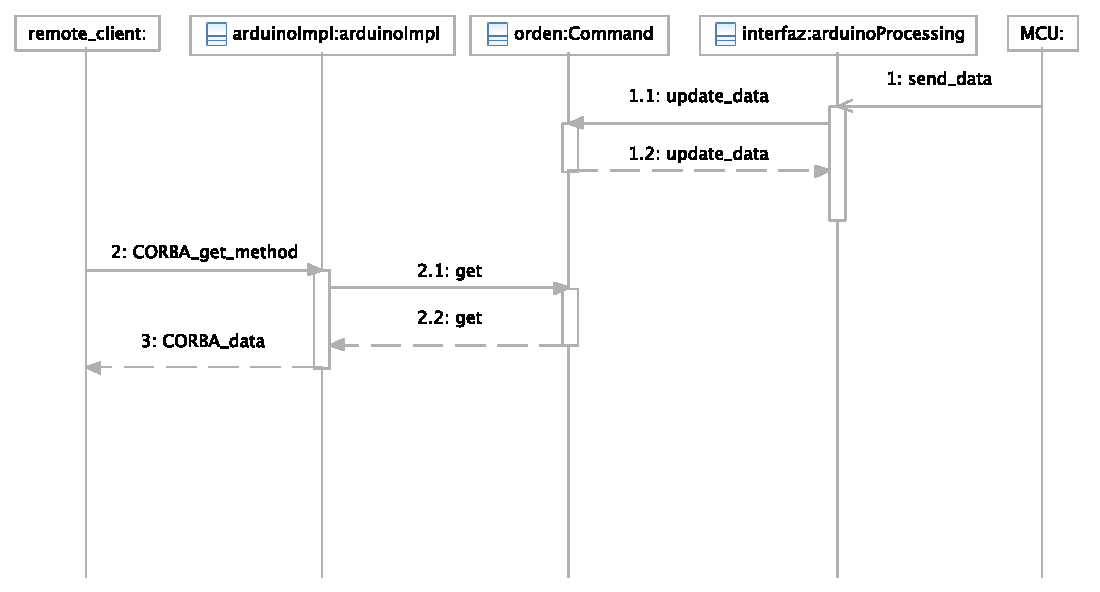
\includegraphics[width=1\textwidth]{RCT_ModulesArduinoA2PC.pdf}}
\end{center}
\caption{Sequence diagram for receiving data from the i/o board.}
\label{fig:ModulesArduinoA2PC}
\end{figure}

\subsubsection{Modifying and uploading the embedded C code}

The embedded program inside the Arduino has been developed using the official IDE
based on the \emph{processing} IDE and the libraries associated to it. A copy of this IDE
can be found inside the source code for the arduino module.

There are a few issues for remembering when installing this module on a fresh
linux installation.
The serial library RXTXcomm is included in the subversion directory \\
\texttt{svn+ssh://sagan/home/svnroot/Higgs/code/devices/arduino/lib}
The file librxtxSerial.so should be copied to \\ \texttt{/usr/\$JAVA\_BASE/jre/lib/i386} and
the three jar files \texttt{core.jar RXTXcomm.jar} and \texttt{serial.jar} to \\
\texttt{/usr/\$JAVA\_BASE/jre/lib/ext}.
Then make sure the user running the servant is in the groups \texttt{uucp}, \texttt{dialout} and
\texttt{lock}, and
that the package uucp is installed. Ensure the cross compilation environment for avr is installed. In Debian/Ubuntu these
are the packages \texttt{gcc-avr}, \texttt{avr-libc} and \texttt{binutils-avr}.

Now check for the embedded C source in the subversion directory
\begin{verbatim}
svn+ssh://sagan/home/svnroot/Higgs/code/\
devices/arduino/arduino\_embedded
\end{verbatim}
A copy of the Integrated Development Environment for the arduino is in
\begin{verbatim}
svn+ssh://sagan/home/svnroot/Higgs/code/devices/\
arduino/arduino-IDE
\end{verbatim}
or you can get the latest version from the web at \\
\texttt{http://arduino.cc/en/Main/Software}.
Start the IDE with \texttt{./arduino} and open the C source file \texttt{arduino\_embedded.pde}.
For the IDE to compile correctly, the name of the source file without the \texttt{.pde}
extension must have the same name as the directory it is in. Select the correct Board and Serial Port
\footnote{The MEGA Arduino board has an integrated USB to RS232 chip, so it will appear as a serial port
\texttt{\/dev\/ttyUSBx} when connecting the USB cable.}
under the \textit{Tools} menu, then Compile/Verify and Upload.

%----------- 5 Power Board ------------

\section{Power board}
\label{sec:devmanual_power}

\begin{figure}[htbp]
\begin{center}
 {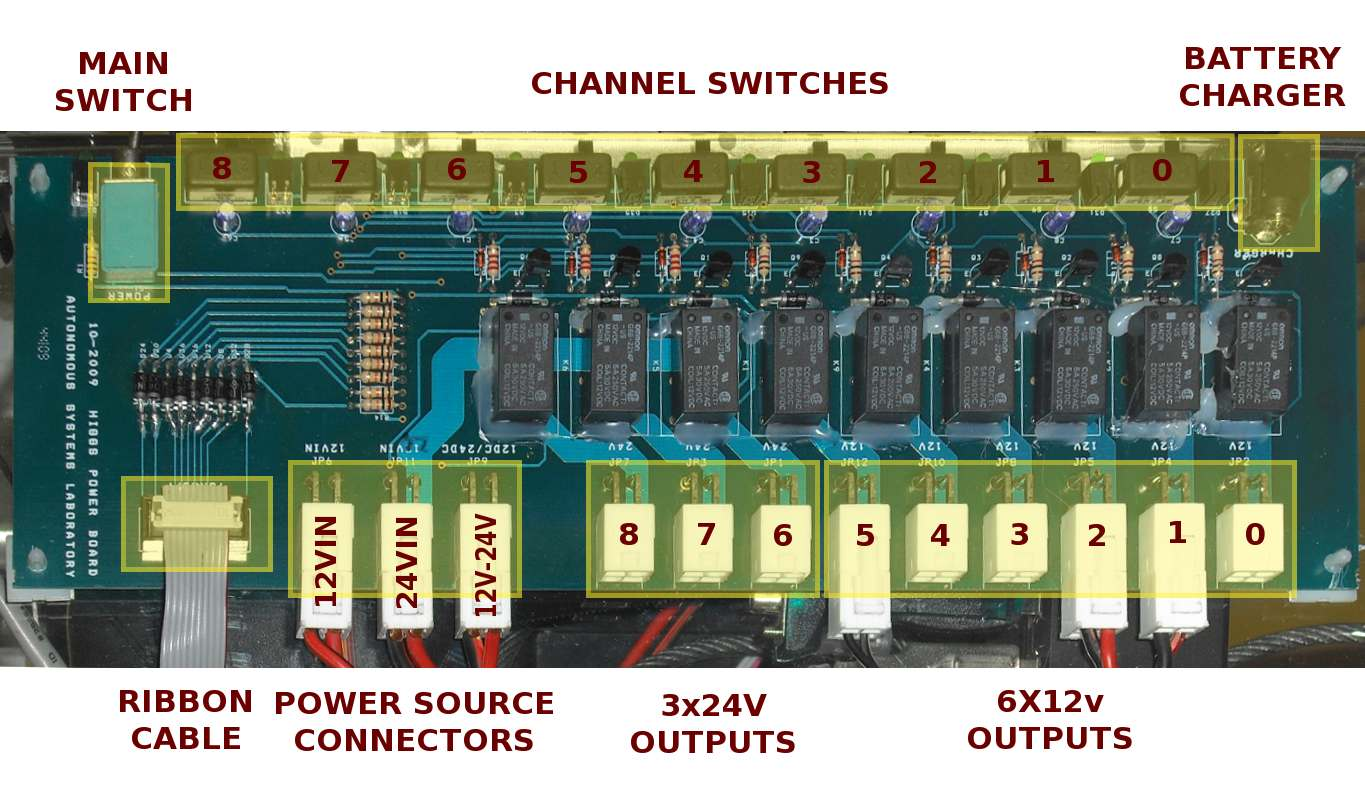
\includegraphics[width=1\textwidth]{RCT_ModulesPowerBoardPhoto.jpg}}
\end{center}
\caption{Photograph of the Power Board indicating each part.}
\label{fig:ModulesPowerBoardPhoto}
\end{figure}
The Power Board is a custom printed circuit board designed specifically for the
needs of the investigators at ASLab with which to test the algorithms in system
auto-reprogramming with partial malfunction of a robot.
The Power Board is in control of the power supply of up to nine devices in the robot. Each
of these channels may be manually shut down by means of a switch or
remotely/automatically using the ribbon cable connection to the Arduino board.
There is a LED power indicator for each channel plus and a switch and LED
indicator for all the board.
Three of the channels, the ones nearer to the general switch, can control 24V
devices whilst the other 6 are for 12V devices. On the back side there are 12
connectors, 6x12V relay controlled outputs, 3x24V relay controlled outputs, 12V
input, 24V input and a 12V output to be taken to the 12VDC to 24VDC converter
that will be powered on whenever any 24V output is enabled. Additionally, there
is a power jack connector for the battery charger\footnote{Originally there was a lead battery pack
for powering the devices on top of the robot base. This power jack connector is no longer neccessary as
the robot base has its own power jack connector for charging the batteries.}.
Thus, the Power Board needs a 12V power source and if the 24V channels are used,
it also needs a 12VDC to 24VDC converter.

\subsection{Power board pinouts}

Check figure \ref{fig:ModulesPowerBoardPhoto} for a visual description of the connectors.
The connector for the ribbon cable has the pinout indicated by table \ref{tab:ModulesArduinoPowerChannels}.
\begin{table}
  \centering
  \begin{tabular}{|c|c|l|} \hline
    \textbf{Channel / Ribbon cable pin} & \textbf{Voltage} & \textbf{Device} \\ \hline \hline
    0  & --- & Ground common \\ \hline
    1  & 12V & Not used \\ \hline
    2  & 12V & Arduino Extension Board (sensors) \\ \hline
    3  & 12V & Servo \\ \hline
    4  & 12V & Kinect \\ \hline
    5  & 12V & GPS receiver \\ \hline
    6  & 12V & Binocular Camera \\ \hline
    7  & 24V & Laser \\ \hline
    8  & 24V & Wrist \\ \hline
    9  & 24V & Not used \\ \hline
  \end{tabular}
  \caption{Distribution of devices in the channels.}
  \label{tab:ModulesArduinoPowerChannels}
\end{table}

The connectors for the devices are Molex MiniFit, RS references 670-5717 (PCB male), 679-5776
(female), 172-9134 (terminals).




\subsection{Electric interface}
The ribbon cable connector has 10 pins. Starting from pin 0, these are ground, the six
12V channels and the three 24V channels.
The channels are shut down writing a logical 0 (0V) to the corresponding pin, whilst
a 1 (5V), a high impedance or a no connection will allow for the channel to be
powered on. Both manual and remote switches must allow for the channel to be
powered on for having that channel powered.

\begin{figure}[htbp]
\begin{center}
 {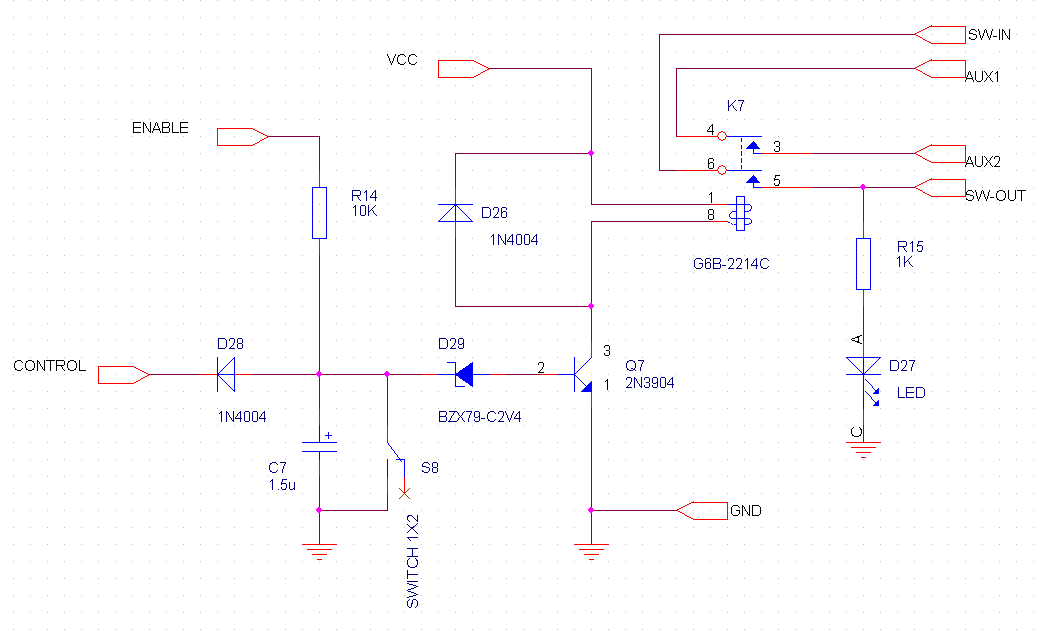
\includegraphics[width=0.9\textwidth]{RCT_ModulesPowerBoardChannelSchematic.png}}
\end{center}
\caption{Schematic for each of the channels.}
\label{fig:ModulesPowerBoardChannelSchematic}
\end{figure}

\begin{figure}[htbp]
\begin{center}
 {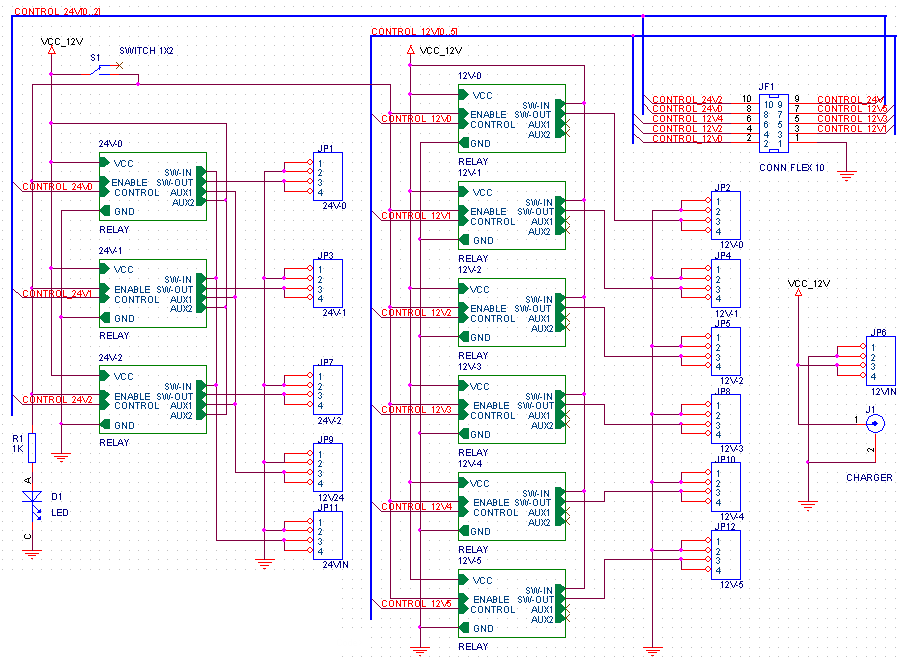
\includegraphics[width=1\textwidth]{RCT_ModulesPowerBoardBlockSchematic.png}}
\end{center}
\caption{Schematic for the Power Board.}
\label{fig:ModulesPowerBoardBlockSchematic}
\end{figure}



\subsection{Power Board Bugs}
During the design phase of the board there were some errors that passed the
internal tests. As the board was to be manufactured once, it was not
economically feasible to built it again and had to be repaired. These bugs
should be revised before sending the design in case the power board should
be manufactured again.
\begin{itemize}
  \item The holes for the diodes 1N4004 are too small. Can be repaired by
    drilling bigger holes and solding the diodes on both sides.
  \item The power jack has the positive pin disconnected. Solved with a bit of
    tin covering both the connected pin hole and the positive pin hole.
  \item The silkscreen of the connector for the 24V input is wrong, it has a
    duplicated 12VIN instead of 24VIN. Solved with a marker-pen.
  \item The relay hole distribution has the two rows of pins too far apart.
    Moreover, the coils had positive and negative pins and was not well
    documented in the datasheet, so the coil pins are swapped. Solved by
    manually separating the pins of the relays and extending the coil pins and
    securing the relays with termoadhesive. A second better approach would have been to
    solder all components on the other side of the board.
  \item Sometimes the relays do not activate correctly and/or the external radio
    emitter for the DGPS interfere with them and turns them off. Even though the
    calculations have been based on the components' specification, $R14$ and
    analogous have been reduced to $5K4\Omega$ for ensuring that enough current
    passes through the relay's coil.
\end{itemize}

%----------- 6 Wrist ------------

\section{Wrist}
\label{sec:devmanual_wrist}
The wrist \footnote{Note that even though the manufacturer calls this device
a powercube, internally we call it wrist.} is a two axis robotics kit module with pan and tilt
movements manufactured by Schunk\textregistered{}. It was
originally bought for use as the tilt mechanism for the laser, but as the center of gravity of
the laser does not match the center of rotation of either axis of the wrist, it
would be a very power hungry method for tilting the laser, given that the laser
is heavy and the power comes from a portable battery system. Moreover, one of
the axis from the wrist would be unused. It was finally decided to use the wrist
for controlling the motion of the camera, even thought it could be achieved with
a smaller controller with minor power requirements.

The manufacturer gives several interfaces for controlling the wrist: Profibus,
CAN and serial. The serial RS-232 bus was chosen over the others because of the
simplicity, the availability of drivers and the sufficient fulfillment of our
requirements. It is connected to the on board computer via a custom made
cable with an intermediate RS-2323 to USB converter. The wrist endpoint
has industry standard serial closings.
\subsection{Wrist servant}
All source code for controlling the wrist is located under
\begin{verbatim}
\$(SVN\_ROOT)/Higgs/branches/CORBA/code/devices/wrist
\end{verbatim} The programs and utilities found there include:
\begin{itemize}
\item Low level library with direct access to serial port.
\item Servant code for the CORBA object.
\item Simple CORBA client to test the functionality and status.
\item Graphical CORBA client for manually teleoperating the wrist with the mouse.
\item Compressed file with the obsolete source code for the wrist, starting
  point but fully rewritten code for the current library.
\item PDF file from the manufacturer describing the serial protocol to the wrist.
\end{itemize}

The sources are all under the \texttt{/src} directory and its documentation can be found
inside the source files.

\begin{figure}[htbp]
\begin{center}
 {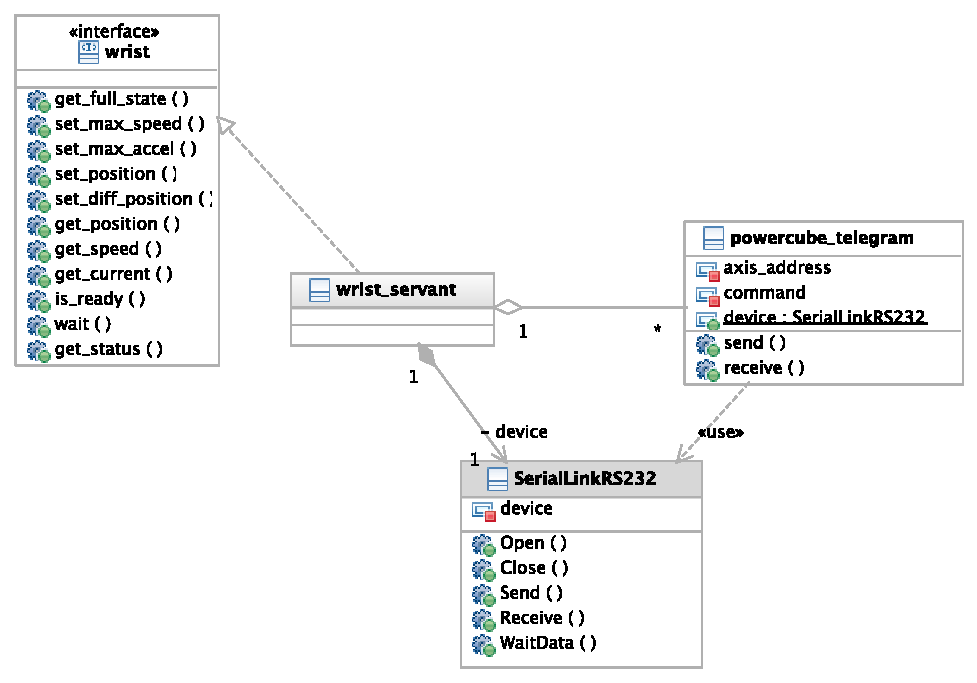
\includegraphics[width=0.95\textwidth]{RCT_ModulesWristClasses.pdf}}
\end{center}
\caption{Class diagram for wrist module and CORBA interface}
\label{fig:ModulesWristClasses}
\end{figure}

\begin{figure}[htbp]
\begin{center}
 {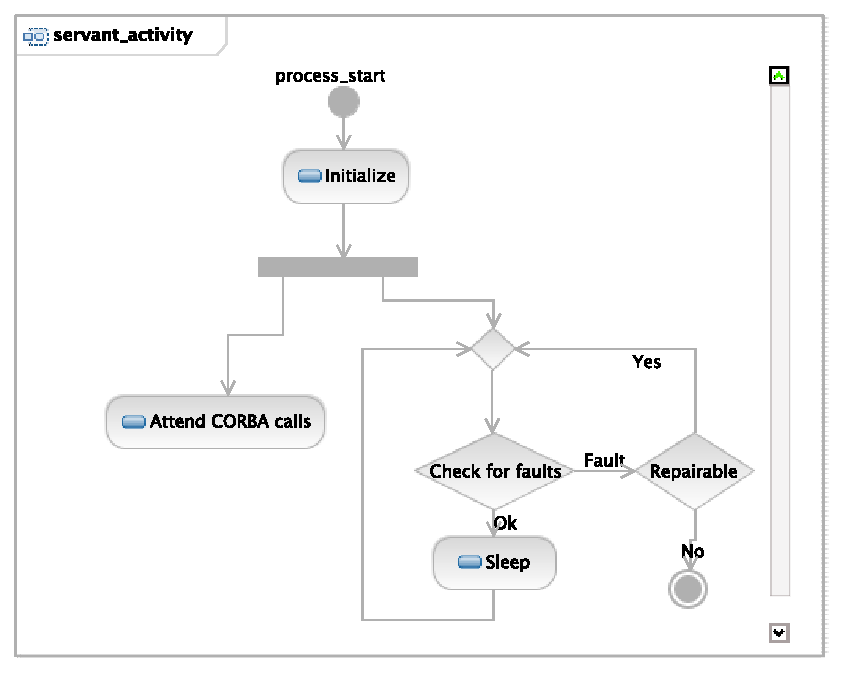
\includegraphics[width=0.95\textwidth]{RCT_ModulesWristActivity.pdf}}
\end{center}
\caption{Activity diagram for wrist servant}
\label{fig:ModulesWristActivity}
\end{figure}

When a CORBA client calls a method of this servant a new telegram is created with the parameters and format adequate to the call, passing the reference to the serial device already initialized. This telegram sends a message to the serial device and waits for the acknowledgement. This is valid for both directions of data flow. The telegram gets destroyed once the communication ends.

\begin{figure}[htbp]
\begin{center}
 {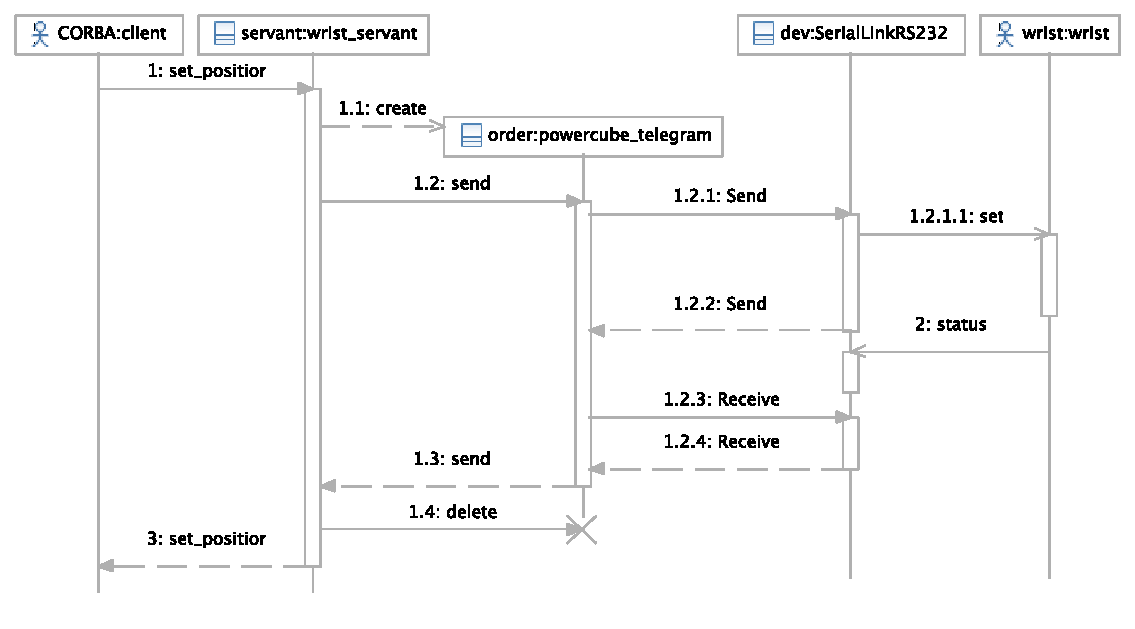
\includegraphics[width=\textwidth]{RCT_ModulesWristCorbaCall.pdf}}
\end{center}
\caption{Sequence diagram for transmitting data to the wrist.}
\label{fig:ModulesWristSequence}
\end{figure}

\subsection{Error recovery}
The wrist must be powered, as said in the official documentation, by  a 24V
power source, mobile or not. However, the fluctuations in voltage caused by
battery charge and the instant consumption of the devices make it difficult to
keep the voltage of the battery near this value. Because of this fact,
the wrist controller has been designed for high error tolerance.
A running thread in the servant polls periodically the wrist for error codes and
takes the appropriate actions when a failure is detected, as explained in each
considered fault.  These are the
possible faults that have been taken into consideration:
\subsubsection{Battery voltage out of bounds}
It has been detected empirically that the wrist will not function if the battery
voltage is under 22V or if it is over 27V, so it will not work if the battery is
either fully charged or next to empty. However, the control electronics are
still available. The status command may be issued to detect this anomaly and a
special status code will be sent by the wrist. The CORBA servant code is aware
of this fault and will abort execution to allow to complete device reset,
outputting a log and leaving the restart of the servant to the VAIO utility
programs. This fault can be prevented by periodically reading
the voltage sensor value from the I/O board, the Arduino CORBA servant.
\subsubsection{Overcurrent}
The internal current sensor will stop the axis when an overcurrent is detected
or a low voltage condition is met if the 12V to 24V converter can not supply
enough power. In this case, a reset and homing procedure is needed before
continuing operating the unit. The maximum speeds and accelerations before the
fault are saved and restored after the reset and homing procedure, but not the
position.
\subsubsection{Device not found}
This error may arise if the device is powered off, if the serial port is not
accessible or can not be found, or if the serial cable is not correctly connected.
In this case the servant will die and get restarted automatically by the init scripts.

%----------- 7 Laser ------------

\section{Laser}
\label{sec:devmanual_laser}

The data cable is a serial one prepared for RS-232 and RS-422 communications.
There is a jumper on the end connector to select which of the protocols to use.
With the jumper, RS-422. Without the jumper, RS-232. Note that the RS-422 has
not been successfully tested, maybe because the jumper should be inside the laser
connection black box instead of the serial cable endpoint.

\subsection{Laser servant}
The laser servant has been developed on top of the driver given by the people working in the mobile robotics lab. It has been modified to be able to resynchronize after a transmission error or a reboot of either the sensor or the servant. The original source code can be found in
\begin{verbatim}
$(SVN)/code/devices/laser/libreria_laser-paloma.zip
\end{verbatim}
The documentation for the Sick Laser Sensor both hardwre and protocol definition can be found under the \texttt{doc} directory of the laser sources. Inside the \texttt{src} directory you will find the modified sources for the laser driver, the servant implementation and a test client, like in other modules.


%----------- 8 Differential GPS ------------

\section{Differential GPS}
\label{sec:devmanual_gps}

The GPS module is based on two OEMV-2-RT2 receptors with capacity for Satellite Based
Augmentation System (SBAS) and Differential GPS (DGPS). Both receptors
communicate through a radio based modem capable of transmitting in half-duplex
mode through relatively long distances at 9600bps. The base radio has a transmitting power of 2W and the
rover radio 0.5W, however the latter is only used for receiving data. Both radios must be set to work in the same channel, use the button with the channel label to change it.
The electronics for each receptor have been encapsulated into plastic boxes with
these connectors and indicators available:
\begin{itemize}
  \item One double power LED indicator for checking 12V and 3.3V.
  \item One USB.
  \item Three RS-232 ports COM1 to COM3 with male DB9 connectors.
  \item One DB9 connector labelled CEXT.
  \item Power Jack connector, 12V nominal.
  \item Two TNC connectors.
  \item A reset button.
\end{itemize}
The connectors used on both base station and rover are the same. The antenna,
either the small one on the rover or the bigger circular one on the base station
is connected to the RFIN-labelled TNC connector. The other TNC connector is not
used and its purpose is to have an external high precission oscillator for the
GPS time measures. The power jack is used to power the unit. COM2 is connected
to the radio emitter/receptor for sending/receiving the differential corrections
from the base station to the rover. COM1 is connected to the VAIO laptop through
a USB to RS232 adaptor so the GPS receiver can send the position information to
the CORBA servant. On the base station, COM1 is only used when configuring the
parameters of the receiver and saving them to its internal non-volatile memory.


\subsection{Configuring the devices}
These procedures are not to be used while on normal operation of the robot. They
are only needed on first boot, then the configuration is saved permanently on
the non-volatile memory of each device. There is a little booklet inside the yellow bag where the station base is stored with the commands and parameters used by the stations.


The \texttt{minicom} command line application is best used. You may have to configure it. Open \texttt{/etc/minirc.ttyS1} and insert these lines:
\begin{verbatim}
 # Machine-generated file - use "minicom -s" to change parameters.
pu port             /dev/ttyS1
pu baudrate         9600
pu bits             8
pu parity           N
pu stopbits         1
pu rtscts           No 
\end{verbatim} 
Change the port as needed.
Run
\begin{verbatim}
 minicom ttyS1
\end{verbatim}
Now you should have access to a command line where you can send commands and check the status of the device.

\subsubsection{Base station}
Set up the base station with the RF input to the external antenna situated in the roof of the department of automatics. Get a serial cable and plug your personal computer to COM1. Start the \texttt{minicom} program to start a new session with the GPS device. These are commands were used to configure it:
\begin{verbatim}
FRESET
FIX POSITION 40.4397076 -3.6881482 744
INTERFACEMODE COM2 NONE CMR OFF
LOG COM2 CMROBS ONTIME 1
LOG COM2 CMRREF ONTIME 10
LOG COM2 CMRDESC ONTIME 10 1
SAVECONFIG
\end{verbatim} 
The meaning of the commands is as follows:
\begin{verbatim}
FRESET
\end{verbatim} 
Clears the non-volatile memory and sets the configuration to the default values. \texttt{RESET} does the same thing without clearing the non-volatile memory.
\begin{verbatim}
FIX POSITION 40.4397076 -3.6881482 744
\end{verbatim} 
This is the position measured for the base station after a period of several hours (Latitude, Longitude, Height). The command indicates the base station that it should calculate the GPS position for the corrections. All position reading after this command returns the fixed coordinates given.
\begin{verbatim}
INTERFACEMODE COM2 NONE CMR OFF
LOG COM2 CMROBS ONTIME 1
LOG COM2 CMRREF ONTIME 10
LOG COM2 CMRDESC ONTIME 10 1
\end{verbatim} 
Sets the COM2 port for sending the corrections using the message types \texttt{CMROBS}, \texttt{CMRREF} and \texttt{CMRDESC}. See the GPS manual for more information. \texttt{ONTIME 1} means to repeat the command every second. Use the \texttt{UNLOG log\_name} and \texttt{UNLOGALL} commands to stop transmitting automatic logs.  Omit \texttt{COM2} for sending the data your terminal.
\begin{verbatim}
SAVECONFIG
\end{verbatim} 
Stores the configuration to the non-volatile memory.

\subsubsection{Rover station}
Proceed as for the base station, except that the serial connection may be already available from the on board computer. In this case you may need to stop the GPS servant first to gain control of the serial device port. These commands were used to configure it:
\begin{verbatim}
FRESET
SBASCONTROL ENABLE EGNOS 0 ZEROTOTWO
INTERFACEMODE COM2 CMR NONE OFF
SAVECONFIG
\end{verbatim}
The \verb|SBASCONTROL| command line configures the GPS mobile station to use the EGNOS/SBAS satellites for better precision than GPS alone if the differential readings are not available.

\subsection{Servant}
The GPS module uses the convention for other module sources: installation and execution procedure, code placement inside the subversion repository and CORBA utilities such as in other modules are used.

The servant code uses non standard commands to receive the data from the rover station.
The commands
\begin{verbatim}
LOG BESTPOS
LOG BESTVEL
\end{verbatim} 
are sent on startup and used to retrieve the information about satellites, position, standard deviation and speed. This data is fetched by an independent thread to the CORBA one and stores it into a shared variable for the CORBA thread to read it each time a client asks for the data. There is also a timeout by which if no data is received after a fixed amount of time an error is issued.

\subsection{Radio signals and ETSII-UPM}
The ETSII-UPM is surrounded by many governmental sites. It is possible that radio transmissions with the differential corrections fail because from interference from these sites. Other investigation groups have had the same problem. In this case the dGPS will not work. Official service has anyway recommended us to use this configuration in the rover if the problem persists:
\begin{verbatim}
UNDULATION USER 0.0
FIX NONE
COM COM2 9600 N 8 1 N OFF
LOG COM2 GPGGA ONTIME logperiod
INTERFACEMODE COM2 CMR NOVATEL OFF
RTKSOURCE type any (ANY)
\end{verbatim}

%----------- 9 Binocular camera ------------

\section{Binocular camera}
\label{sec:devmanual_camera}
The binocular camera is attached to the top of the powercube, allowing for pan
and tilt movements.

The image data is transmitted in raw yuv format between the CORBA servant and the clients.

When restarting the servants, you should kill the process and call \\
\texttt{dc1394\_reset\_bus}, or else the servant will not succeed on starting
again.

\subsection{Compiling and running the CORBA module}
For installing the CORBA module on a fresh fedora linux system, you
must install these libraries which can be found in the repositories
provided by the package \texttt{atrpms}: \texttt{glut glui libavcodec} and
related. Inside the directory tree of the sources there are three scripts that help run the servant and test clients.
Compile and run the server with
\begin{verbatim}
\$ ./1-server.sh
\end{verbatim}
The test client with
\begin{verbatim}
\$ ./2-client.sh
\end{verbatim}
or, for the old client,
\begin{verbatim}
\$ ./3-client.sh
\end{verbatim}
The client runs best when configured to run with Xlib instead of OpenGL.
The user that runs the servant, higgs when running unattended, needs to be in the video group.

The source structure has not been adapted to the new tree configuration nor cmake.
\verb|idl| Contains the idl interfaces. \verb|generated| is where the skeleton and stub source files are generated to. \verb|obj| the binary files are compiled to this directory. \verb|text| contains code to test the camera without using CORBA.


%----------- 10 Other modules ------------

\section{BatteryModel and CurrentMonitor}
\textbf{Note:} Porting to the newer SVN repository is pending.

These two CORBA servants have been implemented into one JAVA binary and made an
unique module inside the VAIO on board computer. The BatteryModel is a component
that calculates the parameters related to the charge in a battery and estimates
the remaining life based on the power requirements. The CurrentMonitor is not
used in any other module but has been an utility component for developing the
BatteryModel. It periodically polls the current of the (currently
instrumentation) batteries and reports the mean consumption since it was
required to start monitoring.

Neither component reads or uses the peripherals on the computer. BatteryModel is
exclusively a CORBA servant and the clients must pass the data to it in order to
compute the estimations for the battery life, whilst CurrentMonitor is, besides
a servant, a client to the Arduino CORBA servant for reading the current values
of the batteries.

Installation of the module and automatic setup is achieved as in the other
modules.




